%% BioMed_Central_Tex_Template_v1.06
%%                                      %
%  bmc_article.tex            ver: 1.06 %
%                                       %

%%IMPORTANT: do not delete the first line of this template
%%It must be present to enable the BMC Submission system to
%%recognise this template!!

%%%%%%%%%%%%%%%%%%%%%%%%%%%%%%%%%%%%%%%%%
%%                                     %%
%%  LaTeX template for BioMed Central  %%
%%     journal article submissions     %%
%%                                     %%
%%          <8 June 2012>              %%
%%                                     %%
%%                                     %%
%%%%%%%%%%%%%%%%%%%%%%%%%%%%%%%%%%%%%%%%%


%%%%%%%%%%%%%%%%%%%%%%%%%%%%%%%%%%%%%%%%%%%%%%%%%%%%%%%%%%%%%%%%%%%%%
%%                                                                 %%
%% For instructions on how to fill out this Tex template           %%
%% document please refer to Readme.html and the instructions for   %%
%% authors page on the biomed central website                      %%
%% http://www.biomedcentral.com/info/authors/                      %%
%%                                                                 %%
%% Please do not use \input{...} to include other tex files.       %%
%% Submit your LaTeX manuscript as one .tex document.              %%
%%                                                                 %%
%% All additional figures and files should be attached             %%
%% separately and not embedded in the \TeX\ document itself.       %%
%%                                                                 %%
%% BioMed Central currently use the MikTex distribution of         %%
%% TeX for Windows) of TeX and LaTeX.  This is available from      %%
%% http://www.miktex.org                                           %%
%%                                                                 %%
%%%%%%%%%%%%%%%%%%%%%%%%%%%%%%%%%%%%%%%%%%%%%%%%%%%%%%%%%%%%%%%%%%%%%

%%% additional documentclass options:
%  [doublespacing]
%  [linenumbers]   - put the line numbers on margins

%%% loading packages, author definitions

\documentclass[twocolumn]{bmcart}% uncomment this for twocolumn layout and comment line below
%\documentclass{bmcart}

%%% Load packages
\usepackage{amsthm,amsmath}
\usepackage{siunitx}
\usepackage{mfirstuc}
%\RequirePackage{natbib}
\usepackage[colorinlistoftodos]{todonotes}
\RequirePackage{hyperref}
\usepackage[utf8]{inputenc} %unicode support
%\usepackage[applemac]{inputenc} %applemac support if unicode package fails
%\usepackage[latin1]{inputenc} %UNIX support if unicode package fails
\usepackage[htt]{hyphenat}

\usepackage{array}
\newcolumntype{L}[1]{>{\raggedright\let\newline\\\arraybackslash\hspace{0pt}}p{#1}}

%%%%%%%%%%%%%%%%%%%%%%%%%%%%%%%%%%%%%%%%%%%%%%%%%
%%                                             %%
%%  If you wish to display your graphics for   %%
%%  your own use using includegraphic or       %%
%%  includegraphics, then comment out the      %%
%%  following two lines of code.               %%
%%  NB: These line *must* be included when     %%
%%  submitting to BMC.                         %%
%%  All figure files must be submitted as      %%
%%  separate graphics through the BMC          %%
%%  submission process, not included in the    %%
%%  submitted article.                         %%
%%                                             %%
%%%%%%%%%%%%%%%%%%%%%%%%%%%%%%%%%%%%%%%%%%%%%%%%%


%\def\includegraphic{}
%\def\includegraphics{}

%%% Put your definitions there:
\startlocaldefs
\endlocaldefs


%%% Begin ...
\begin{document}

%%% Start of article front matter
\begin{frontmatter}

\begin{fmbox}
\dochead{Report from 2015 Brainhack Americas (MX)}

%%%%%%%%%%%%%%%%%%%%%%%%%%%%%%%%%%%%%%%%%%%%%%
%%                                          %%
%% Enter the title of your article here     %%
%%                                          %%
%%%%%%%%%%%%%%%%%%%%%%%%%%%%%%%%%%%%%%%%%%%%%%

\title{NeuroView: a customizable browser-base utility}
\vskip2ex
\projectURL{Project URL: \url{https://github.com/lsa-pucrs/neuroview}}

\author[
addressref={pucrs},
%
email={anibalsolon@gmail.com}
]{\inits{ASH} \fnm{Anibal} \snm{Sólon Heinsfeld}}
\author[
addressref={pucrs},
%
email={alexandre.franco@pucrs.br}
]{\inits{ARF} \fnm{Alexandre} \snm{Rosa Franco}}
\author[
addressref={pucrs},
%
email={augusto.buchweitz@pucrs.br}
]{\inits{AB} \fnm{Augusto} \snm{Buchweitz}}
\author[
addressref={pucrs},
%
email={felipe.meneguzzi@pucrs.br}
]{\inits{FM} \fnm{Felipe} \snm{Meneguzzi}}

%%%%%%%%%%%%%%%%%%%%%%%%%%%%%%%%%%%%%%%%%%%%%%
%%                                          %%
%% Enter the authors' addresses here        %%
%%                                          %%
%% Repeat \address commands as much as      %%
%% required.                                %%
%%                                          %%
%%%%%%%%%%%%%%%%%%%%%%%%%%%%%%%%%%%%%%%%%%%%%%

\address[id=pucrs]{%
  \orgname{PUCRS},
  \city{Porto Alegre},
  \street{Av. Ipiranga, 6681},
  \postcode{90619-900},
  \postcode{Rio Grande do Sul},
  \cny{Brazil}
}

%%%%%%%%%%%%%%%%%%%%%%%%%%%%%%%%%%%%%%%%%%%%%%
%%                                          %%
%% Enter short notes here                   %%
%%                                          %%
%% Short notes will be after addresses      %%
%% on first page.                           %%
%%                                          %%
%%%%%%%%%%%%%%%%%%%%%%%%%%%%%%%%%%%%%%%%%%%%%%

\begin{artnotes}
\end{artnotes}

%\end{fmbox}% comment this for two column layout

%%%%%%%%%%%%%%%%%%%%%%%%%%%%%%%%%%%%%%%%%%%%%%
%%                                          %%
%% The Abstract begins here                 %%
%%                                          %%
%% Please refer to the Instructions for     %%
%% authors on http://www.biomedcentral.com  %%
%% and include the section headings         %%
%% accordingly for your article type.       %%
%%                                          %%
%%%%%%%%%%%%%%%%%%%%%%%%%%%%%%%%%%%%%%%%%%%%%%

%\begin{abstractbox}

%\begin{abstract} % abstract
	
%Blank Abstract

%\end{abstract}



%%%%%%%%%%%%%%%%%%%%%%%%%%%%%%%%%%%%%%%%%%%%%%
%%                                          %%
%% The keywords begin here                  %%
%%                                          %%
%% Put each keyword in separate \kwd{}.     %%
%%                                          %%
%%%%%%%%%%%%%%%%%%%%%%%%%%%%%%%%%%%%%%%%%%%%%%

%\vskip1ex

%\projectURL{\url{https://github.com/lsa-pucrs/neuroview}}
%\projectURL{https://github.com/lsa-pucrs/neuroview}

% MSC classifications codes, if any
%\begin{keyword}[class=AMS]
%\kwd[Primary ]{}
%\kwd{}
%\kwd[; secondary ]{}
%\end{keyword}

%\end{abstractbox}
%
\end{fmbox}% uncomment this for twcolumn layout

\end{frontmatter}

%{\sffamily\bfseries\fontsize{10}{12}\selectfont Project URL: \url{https://github.com/lsa-pucrs/neuroview}}

%%% Import the body from pandoc formatted text
\section{Introduction}\label{introduction}

The amount of data acquired for an fMRI experiment dimension wise is
very large and a challenge for neuroscience studies, in particular for
data analysis and visualization. There are different tools developed to
address such massive data challenges, in particular, the analysis needs
for different projects may require new tools. The goal of this Brainhack
project is to build a flexible utility to analyze fMRI experimental
results. This utility is called NeuroView. NeuroView allows researchers
to extend the visualizations to their context: every visual behavior or
interactions of this tool is customizable. We implemented NeuroView to
work in Web-browsers, using JavaScript and the libraries D3.js and
jQuery.

\section{Results}\label{results}

We create three tools using NeuroView to best analyze research results:
CC200 search, SVM coeffs and Connectivity matrix. Each tool is used to
aid the analysis of results in Machine Learning tasks. Each of these
tools is described below in detail.

\subsection{\texorpdfstring{\texttt{CC200 search}:}{:}}\label{section}

In this tool, we allow the user to find atlas regions (e.g.~Left Putamen
from Harvard-Oxford subcortical structural atlas) mapped to a specific
parcellation. As as initial approach, the CC200 \cite{Craddock2012}
parcellation method was used, since our analysis uses data from
functional MRI. Since we parcellate our data into CC200's ROIs in most
of our studies, the identification of atlas regions became necessary to
compare with results found in the literature. The search can be
performed in two manners: it is possible to search for an atlas region
(e.g.~Putamen) and retrieve which parcels are included in this region,
and it is possible to click an ROI in NeuroView to retrieve which atlas
regions include the specific parcel.

\subsection{\texorpdfstring{\texttt{SVM coeffs}:}{:}}\label{section-1}

For the second tool, we created a user interface to identify the ROIs
that contribute to the classification in a Support Vector Machine. The
classification method uses task-based fMRI features to identify good and
poor readers \cite{Salles2013}. Given a list of most relevant features,
as shown in Figure \ref{fig:svm_coeffs}, we can show the features'
parcel in NeuroView and identify to which atlas regions this parcel
belongs to.

\begin{figure}[ht]
\centering
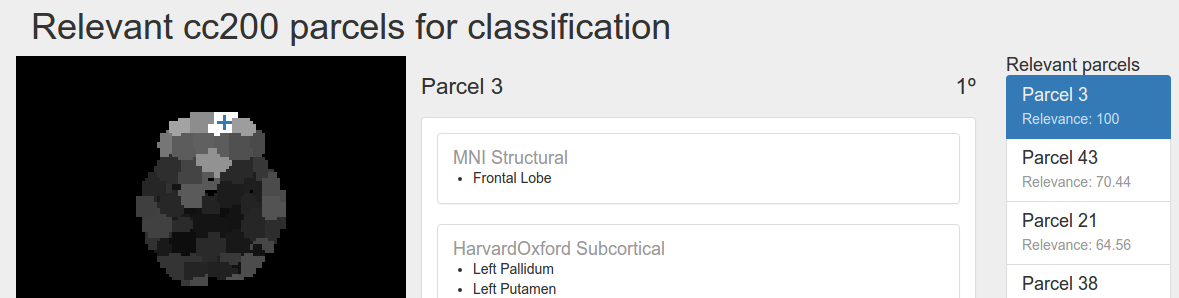
\includegraphics[width=0.45\textwidth]{figs/svm_coeffs.png}
\caption{SVM coeffs tool showing the most relevant feature in a classification task.}
\label{fig:svm_coeffs}
\end{figure}

\subsection{\texorpdfstring{\texttt{Connectivity matrix}:}{:}}\label{section-2}

In the third study case, NeuroView was customized to interact with a
connectivity chord plot (or connectogram) \cite{Irimia2012}. This plot
contains each CC200 parcel and chords that represent the connectivity
between these parcels. Since we use the connectivity matrix as features
for our deep learning method, we need to check which feature (i.e.~the
correlation between two parcels) most contributes to the classification.
After thresholding 17995 features, we retrieve ten features that are
more relevant in our analysis, as shown in Figure
\ref{fig:deeplearning}. In the chord plot, a red chord indicates that
two regions are correlated, and a blue chord indicates that two regions
are anti-correlated. By clicking a chord, NeuroView highlights the
regions that are connected by this chord. Thus, highlighted regions are
correlated (or anti-correlated) given the chord color.

\begin{figure}[ht]
\centering
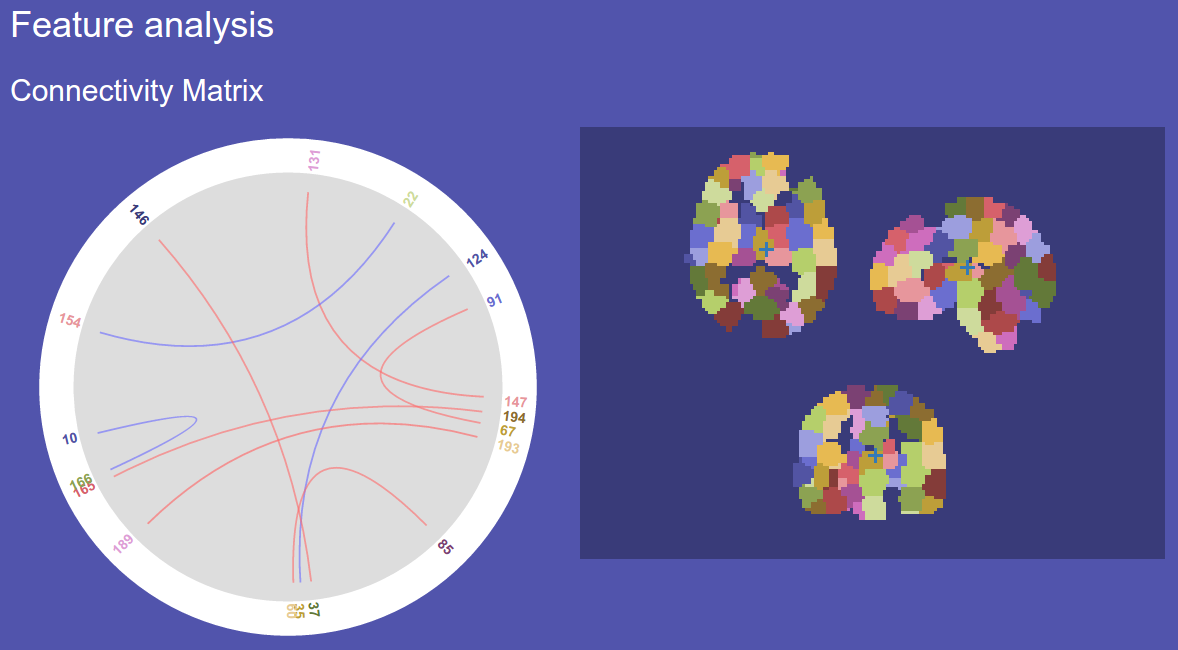
\includegraphics[width=0.45\textwidth]{figs/deeplearning.png}
\caption{Deep learning.}
\label{fig:deeplearning}
\end{figure}

\section{Conclusion}\label{conclusion}

This is an initial version of a browser-based neuroimage viewer. The
main focus is to develop an embeddable viewer, instead of a standalone
desktop software. By doing so, research results can be presented on
interactive views, enriching their analysis and interpretation. In our
case study, NeuroView facilitates quick evaluation of features for
machine learning algorithms, and promote discussion about them, since
the results were enlightened among researchers.

As further work, we aim to directly load Nifti images at client-side and
support some AFNI's features, such as voxel clustering.

%%%%%%%%%%%%%%%%%%%%%%%%%%%%%%%%%%%%%%%%%%%%%%
%%                                          %%
%% Backmatter begins here                   %%
%%                                          %%
%%%%%%%%%%%%%%%%%%%%%%%%%%%%%%%%%%%%%%%%%%%%%%

\begin{backmatter}

\section*{Availability of Supporting Data}
More information about this project can be found at: \url{https://github.com/lsa-pucrs/neuroview}. Further data and files supporting this project are hosted in the \emph{GigaScience} repository REFXXX.

\section*{Competing interests}
None

\section*{Author's contributions}
ASH wrote the software, and ASH, FM, ARF, and AB wrote the report.

\section*{Acknowledgements}
The authors would like to thank the organizers and attendees of
Brainhack MX and the developers of AFNI.

  
  
%%%%%%%%%%%%%%%%%%%%%%%%%%%%%%%%%%%%%%%%%%%%%%%%%%%%%%%%%%%%%
%%                  The Bibliography                       %%
%%                                                         %%
%%  Bmc_mathpys.bst  will be used to                       %%
%%  create a .BBL file for submission.                     %%
%%  After submission of the .TEX file,                     %%
%%  you will be prompted to submit your .BBL file.         %%
%%                                                         %%
%%                                                         %%
%%  Note that the displayed Bibliography will not          %%
%%  necessarily be rendered by Latex exactly as specified  %%
%%  in the online Instructions for Authors.                %%
%%                                                         %%
%%%%%%%%%%%%%%%%%%%%%%%%%%%%%%%%%%%%%%%%%%%%%%%%%%%%%%%%%%%%%

% if your bibliography is in bibtex format, use those commands:
\bibliographystyle{bmc-mathphys} % Style BST file
\bibliography{brainhack-report} % Bibliography file (usually '*.bib' )

\end{backmatter}
\end{document}
